% TEX STUDIO MAGIC-COMMAND
% !TeX document-id = {21ffa6e2-6c8f-4532-897c-386dc477f19a}
% !TeX root = abstract.tex
%%% ↑ TeXのファイル名にあわせること.
% !TeX encoding = utf8
% !TeX TXS-program:compile = lualatex -synctex=1 -interaction=nonstopmode -halt-on-error %.tex
% !TeX TXS-program:quick = txs:///compile | txs:///view-pdf-internal --embedded

%%%-------------------------------------------------------------------------
%%% PD3予稿集テンプレート (main.tex)
%%% 作成: 金沢工大・情報工学科・鷹合研究室(2022,01/12)
%%%-------------------------------------------------------------------------

%%%%%%%%%%%%%%%%%%%%%%%%%%%%%%%%%%%%%%%%%%%%%%%%%%%%%%%%%%%%%%%%%%%%%%%%%%%
%                               テーマ,著者情報をここに書き込んでください
%ここから ------------------------------------------------------------------

%%% テーマ番号
\def\THEMEID{坂本研-04}

%%% タイトル
\def\TITLEJP{観光案内アプリにおけるPWAの活用に関する検討}
\def\TITLEEN{A Study on the Use of PWA in Tourist Information Apps}
\def\CENTERADJ{2.2} % ここを書き換えて,表紙の「プロジェクトテーマ」という文字列がセル中心になるよう調整してください

%%% 教員名
\def\PROFNAME{坂本 真仁 講師}

%%% アブストラクト(英文で書く)
% 最低:100ワード,最大:300ワード前後
% 英文部分については,句読点は半角にすること.つまり", "か". "を使う
\def\ABSTRACT{
With the spread of mobile devices such as smartphones, native mobile applications are now used by many people. Such native applications provide functions such as caching for faster loading and offline access. Developers can use these features to reduce data traffic and improve user experience. Progressive Web Apps(PWA) can be used to implement similar functionality in web applications. The advantages and challenges of PWA in tourist information applications will be evaluated by comparing them with native and regular web applications.
}

%%% キーワード(5個まで)
\def\KEYWORDS{Progressive Web Apps, Mobile}

%%% 著者リスト
\def\AUTHORS{
\begin{minipage}{13.5cm}
4EP1-25~笹川 尋翔(SASAGAWA Hiroto)
\end{minipage}
}

% テーマ,著者情報ここまで -----------------------------------------------------


%%%%%%%%%%%%%%%%%%%%%%%%%%%%%%%%%%%%%%%%%%%%%%%%%%%%%%%%%%%%%%%%%%%%%%%%%%%%
%                                本文
\documentclass{tkglabs}

\begin{document}
\maketitle
\begin{multicols*}{2} % *アスタ付きだとページのバランシングを無効にできる
%本文ここから ------------------------------------------------------------------

\section{背景}
情報端末の普及や多様化に伴い、特定のアプリプラットフォームに依存しないシステムであるWebが果たすべき役割が拡大している。この影響を受けて、現在はWHATWGやW3CによるWebの標準化が進められており、WebAssemblyによる処理の高速化やWeb APIによる高度な画像/動画処理が実現できるようになるなどの進展が見られる。モバイル端末において利用できるアプリとして、主にネイティブアプリケーションとWebアプリケーションがある。

ネイティブアプリケーションは一般的に、アプリストアと呼ばれる、ユーザーがアプリをダウンロードしたり購入したりするプラットフォームからダウンロードされ、インストールされる。ネイティブアプリケーションの長所は、オフラインアクセスが利用できる、カメラやプッシュ通知などのモバイル端末の機能にアクセスできる、適切な設計を行うことでWebアプリケーションよりも優れたユーザー体験を提供できる点である。

Webアプリケーションは、Webブラウザ上で動作するアプリである。Webアプリケーションの長所は、アプリのインストールが不要である、アプリのサイズがネイティブアプリケーションよりも小さい、更新がすぐに行われる点である。

2015年にProgressive Web Apps(PWA)という技術が登場した。これを活用することで、Webアプリケーションにおいてプッシュ通知、オフラインアクセス、ホーム画面へのロードなどの機能をネイティブアプリケーションと同じように利用できる。表~\ref{table1}に、PWAとネイティブアプリケーション、およびWebアプリケーションのそれぞれの特徴を示す。

\begin{table*}
  \centering
  \tabcap{モバイル端末で利用できる主なアプリの特徴}{Main app features available on mobile devices}{}
  \label{table1}
\begin{tabular}{|p{10em}|p{10em}|p{10em}|p{10em}|}
\hline
          & ネイティブアプリケーション & PWA    & 通常のWebアプリケーション      \\ \hline
インストール方法    & アプリストアにアクセス   & ``ホーム画面に追加する''ボタンを選択 & できない                \\ \hline
アップデート方法    & アプリストアにアクセス  & ページを再読み込み            & ページを再読み込み        \\ \hline
クライアント側で保持するファイルサイズ       & 大きい           & 小さい                     & 小さい                 \\ \hline
ユーザー体験    & 良い & 比較的良い     & 比較的悪い \\ \hline
プッシュ通知    & できる           & できる                     & サードパーティーのサービスを利用 \\ \hline
オフラインアクセス & できる           & できる                     & できない                \\ \hline
\end{tabular}
\end{table*}

モバイル端末が広く活用されるようになったことで、観光客の利便性向上を目的とした観光案内アプリも数多くリリースされている。日本においては、青森市\cite{AomoriCityTravelNavi}、 長野県\cite{ShinshuNavi}、和歌山市\cite{WakayamaSightseeing}などの様々な自治体が観光案内アプリを提供している。このようなアプリの特徴の1つとして、大量の画像、動画、音声などのコンテンツを扱うことが挙げられる。モバイル端末は、必ずしも高速で安定したネットワーク環境において使用されるとは限らないため、大量のコンテンツを効率良く扱うためにはキャッシュの管理が有効である。また、観光案内の役割を果たすために、プッシュ通知を通じて観光客の活動を促進することも重要である。これらの機能をPWAを用いて実装することで、開発工数を削減したり、Webアプリケーション開発の知識を活用したりできる。

\section{関連研究}
Tandelらの論文では、PWAの構成要素としてApp Shell、Service Worker、マニフェストがあることが示されている\cite{Tandel2018ProgressiveWebApps}。PWAでは、コンテンツから分離されたアプリのUIを``シェル''という。App ShellはシェルをキャッシュすることでWebアプリケーションをオフライン環境で快適に動作させるためのモデルである。Service Workerはバックグラウンドタスクを処理するためのエントリーポイントとして動作するスレッドを実行するモジュールである。マニフェストはアプリに関する情報を提供するファイルであり、アプリの名前、説明、作者、アイコンのパスをJSONテキストファイルに記述したものである。

Majchrzakらの論文では、クロスプラットフォーム開発が依然として重要なテーマであることを述べた上で、実例に基づいた研究によって、PWAの利便性がどの程度であるかを明らかにすることを今後の課題として挙げている\cite{Majchrzak2018ProgressiveWebApps}。2023年3月28日にリリースされたiOS 16.4でPWAのプッシュ通知に対応するなどの変更があったため、この研究では、最新の情報を元に改めてiOSにおけるPWAへの対応状況を説明する。

\section{目的}
観光案内アプリという実例に基づいて、PWAの利便性の程度を明らかにする。PWAは、ネイティブアプリケーションに近い動作をWebアプリで実現するものである。そこでこの研究では、PWAの利便性は、ネイティブアプリケーションで利用できる機能との互換性とPWAのパフォーマンスに基づくと解釈して、PWAを用いて実装した観光案内アプリの利便性を評価する。

\section{アプリの概要}
まず、観光案内アプリとして満たすべき機能を整理する。初めに必要とされる機能は、公共交通機関と観光名所の場所を示すことである。一般的に地図アプリを用いてこの機能を実装することが多いため、このアプリでは、Google MapsにGeoJSONデータをインポートしてそれらの場所を示す。GeoJSONとは、地理的データを表すJSONオブジェクトである。公共交通機関と観光名所のGeoJSONデータは、Overpass turbo\cite{OverpassTurbo}から取得する。Overpass turboは、Overpass APIを使用してOpenStreetMapのデータを取得できるWebサービスである。

地図に示された場所をユーザーが選択した際に詳細を表示する機能も必要である。詳細ページでは、JSONPlaceholder\cite{JSONPlaceholder}から取得した画像とテキストを表示する。JSONPlaceholderは、ダミーデータを提供するAPIである。作成するアプリの画面遷移図を図~\ref{figure1}に示す。

\begin{figure}
  \centering
  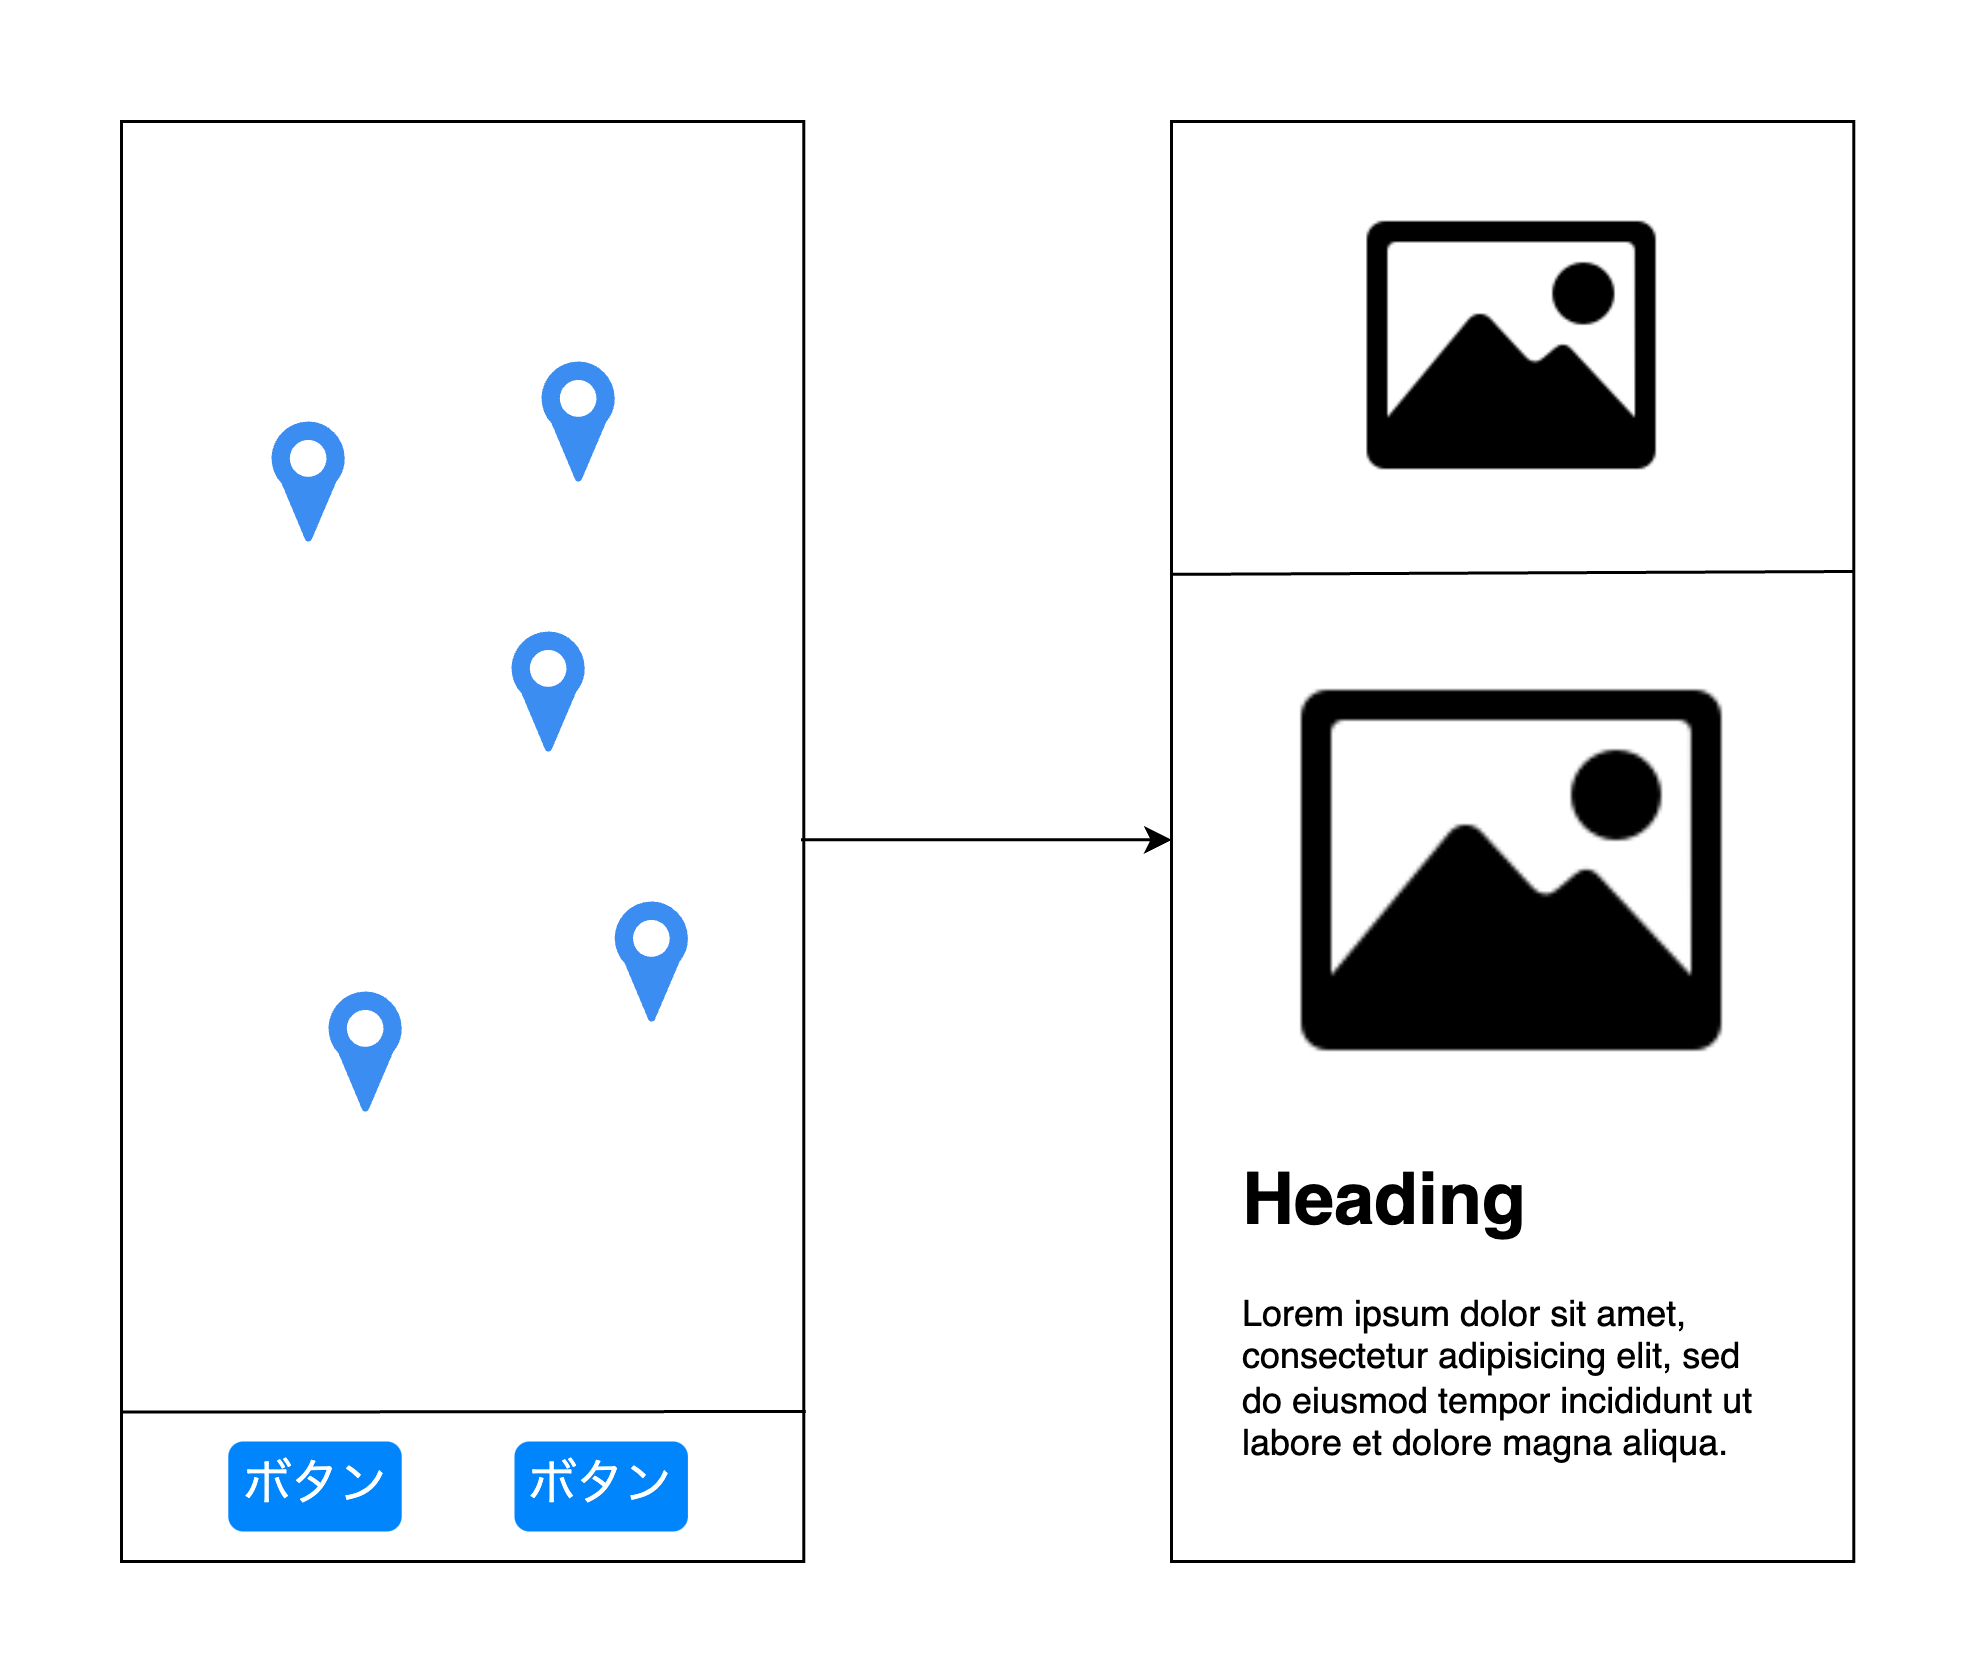
\includegraphics[width=\linewidth]{fig/screen_transition_diagram.png}
  \figcap{作成するアプリの画面遷移図}{Screen transition diagram of the application to be created}{}
  \label{figure1}
\end{figure}

\section{評価方法}
初めに、オフラインアクセス、キャッシュ、プッシュ通知などの機能の処理の流れを、ネイティブアプリケーション、PWA、通常のWebアプリケーションの間で比較する。次に、Lighthouse\cite{Lighthouse}というベンチマークツールを用いて、PWAと通常のWebアプリケーションのパフォーマンスの違いを計測する。Lighthouseでは、ネットワークやCPUの速度などをエミュレートしてパフォーマンスを計測したり、リクエストやレスポンスの内容を確認したりできる。
動作確認に用いる端末は以下の通りである。モバイル端末のOSごとにPWAの動作が異なるため、複数の端末を使用して動作を確認する。

\begin{itemize}
  \item motorola edge 20 fusion
    \begin{itemize}
      \item OS: Android 12
    \end{itemize}
  \item iPhone SE 第2世代
    \begin{itemize}
      \item OS: iOS 16.5
    \end{itemize}
\end{itemize}

\section{今後の展望}
実際の観光案内アプリにおいて、SDKを用いて実装されている機能を調査する。それと平行して、PWAを組み込むためのWebアプリケーションを作成する。作成したWebアプリケーションのパフォーマンスを適切に評価するために、Lighthouseで測定できる指標とその概要を調査することも必要である。また、Lighthouseではネットワークエミュレーションを使用した評価も行うため、基地局の性能や回線エリアのカバー率に関する最新の情報を調査して、エミュレートする回線速度を検討することも今後の課題である。

%% 参考文献(必要に応じて追加)
\begin{thebibliography}{9}
\bibitem{AomoriCityTravelNavi} 青森市, ``青森市観光ナビゲーションアプリ「青森市観光ナビ」-Aomori City Travel Navi-のご案内,'' \url{https://www.city.aomori.aomori.jp/kouryuu-suishin/kannkonabi.html} (2023年9月1日アクセス).
\bibitem{ShinshuNavi} 長野県, ``信州ナビ,'' \url{https://shinshu-navi.net/lp/} (2023年9月1日アクセス).
\bibitem{WakayamaSightseeing} 和歌山市, ``和歌山市観光アプリ,'' \url{http://www.city.wakayama.wakayama.jp/kankou/kankouspot/1027585/1027586.html} (2023年9月1日アクセス).
\bibitem{Tandel2018ProgressiveWebApps} S. S. Tandel and A. Jamadar, ``Impact of Progressive Web Apps on Web App Development,'' \textit{International Journal of Innovative Research in Science, Engineering and Technology}, vol. 7, pp. 9439-9444, Sep. 2018.
\bibitem{Majchrzak2018ProgressiveWebApps} T. A. Majchrzak \textit{et al.}, ``Progressive Web Apps: the Definite Approach to Cross-Platform Development?,'' in \textit{Proceedings of the 51st Hawaii International Conference on System Sciences}, IEEE Computer Society, Jan. 2018. pp. 5735-5744. 
\bibitem{OverpassTurbo} M. Raifer, ``overpass turbo,'' \url{https://overpass-turbo.eu/} (2023年9月1日アクセス).
\bibitem{JSONPlaceholder} typicode, ``JSONPlaceholder - Free Fake REST API,'' \url{https://jsonplaceholder.typicode.com/} (2023年9月11日アクセス).
\bibitem{Lighthouse} Chrome Developers, ``Lighthouse,'' \url{https://developer.chrome.com/docs/lighthouse/} (2023年9月1日アクセス).
\end{thebibliography}

% 本文ここまで ------------------------------------------------------------------
\end{multicols*}
\end{document}
